\chapter{Graph Basics, BFS and DFS}

\tikzset{gv/.style={circle, draw, thick, minimum size=6.5mm, inner sep=0pt, font=\small},
  ge/.style={thick}, gd/.style={thick, -{Stealth[length=2.2mm]}}}

\section{Definitions and representations}
A graph $G=(V,E)$ has $n=|V|$ vertices and $m=|E|$ edges. In an undirected graph, $m\le\binom n2$; in a directed graph, $m\le n(n-1)$.
A graph is \emph{connected} if every pair of vertices is joined by a path; a \emph{tree} is a connected acyclic graph (with $n-1$ edges).

\begin{center}
\begin{tabular}{lll}
\toprule
 & Adjacency matrix & Adjacency lists \\
\midrule
Space & $\Theta(n^2)$ & $\Theta(n+m)$ \\
Is $(u,v)\in E$? & $\Theta(1)$ & $\Theta(\deg u)$ \\
List neighbours of $u$ & $\Theta(n)$ & $\Theta(\deg u)$ \\
\bottomrule
\end{tabular}
\end{center}
We use adjacency lists unless stated; ``linear time'' for graphs means $\bigO(n+m)$.
Handshake lemma: $\sum_v\deg(v)=2m$.

\section{Breadth-first search}
BFS explores vertices in order of distance (number of edges) from a source $s$.
\begin{lstlisting}[style=pseudo]
BFS(G, s):
    for each v in V do dist[v] = $\infty$; parent[v] = nil
    dist[s] = 0; Q = queue containing s
    while Q not empty do
        u = Dequeue(Q)
        for each v adjacent to u do
            if dist[v] == $\infty$ then
                dist[v] = dist[u] + 1; parent[v] = u; Enqueue(Q, v)
\end{lstlisting}
Each vertex is enqueued at most once and each adjacency list scanned once: $\bigO(n+m)$.

\begin{theorem}
After BFS, $\mathrm{dist}[v]=\delta(s,v)$, the length of a shortest $s$-$v$ path, and following \code{parent} pointers gives a shortest path.
\end{theorem}
\begin{proof}[Proof sketch]
Invariant: the queue holds vertices with nondecreasing \code{dist}, and the first and last differ by at most 1.
So vertices are dequeued in nondecreasing order of \code{dist}. Clearly $\mathrm{dist}[v]\ge\delta(s,v)$ since it is the length of an
actual path. Suppose $v$ is a vertex with minimum $\delta(s,v)$ such that $\mathrm{dist}[v]>\delta(s,v)$, and let $u$ be the vertex before $v$
on a shortest path; then $\mathrm{dist}[u]=\delta(s,u)=\delta(s,v)-1$. When $u$ was dequeued, $v$ was either undiscovered (then
$\mathrm{dist}[v]=\mathrm{dist}[u]+1$) or already discovered from a vertex dequeued no later than $u$, giving $\mathrm{dist}[v]\le\mathrm{dist}[u]+1$. Contradiction.
\end{proof}

The parent edges form the \textbf{BFS tree}. In an undirected graph every non-tree edge joins vertices whose levels differ by at most 1.

\begin{figure}[H]
\centering
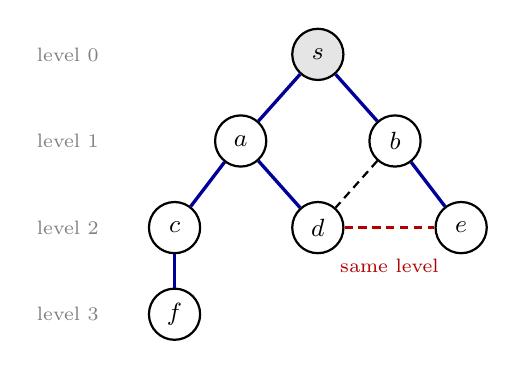
\begin{tikzpicture}[x=1.4cm, y=1.1cm]
  \foreach \l in {0,1,2,3} \node[font=\scriptsize, gray, anchor=east] at (-0.4,-\l) {level \l};
  \node[gv, fill=gray!20] (s) at (1.5,0) {$s$};
  \node[gv] (a) at (0.8,-1) {$a$};
  \node[gv] (b) at (2.2,-1) {$b$};
  \node[gv] (c) at (0.2,-2) {$c$};
  \node[gv] (d) at (1.5,-2) {$d$};
  \node[gv] (e) at (2.8,-2) {$e$};
  \node[gv] (f) at (0.2,-3) {$f$};
  \foreach \u/\v in {s/a, s/b, a/c, a/d, b/e, c/f} \draw[ge, very thick, blue!60!black] (\u) -- (\v);
  \draw[ge, densely dashed] (b) -- (d);
  \draw[ge, red!70!black, densely dashed] (d) -- (e);
  \node[font=\scriptsize, red!70!black, anchor=north] at (2.15,-2.25) {same level};
\end{tikzpicture}
\caption{BFS from $s$: tree edges (solid) and non-tree edges (dashed), which
join equal or adjacent levels. The edge $de$ joins two vertices of level 2,
so $b,d,e$ form an odd cycle and the graph is not bipartite.}
\end{figure}

\subsection{Testing bipartiteness}
$G$ is \emph{bipartite} if $V=A\cup B$ with every edge between $A$ and $B$; equivalently, $G$ is 2-colourable.
\begin{theorem}
A graph is bipartite if and only if it has no odd cycle.
\end{theorem}
\textbf{Algorithm}: run BFS from each unvisited vertex; colour by parity of level. If some edge joins two vertices of the same level,
report ``not bipartite'', otherwise the colouring is a valid bipartition. $\bigO(n+m)$.

\begin{proof}[Correctness]
If no edge joins same-level vertices, all edges join adjacent levels (BFS property), which have different parities: valid 2-colouring.
If edge $uv$ joins two vertices at the same level $k$, let $w$ be their lowest common ancestor in the BFS tree at level $j<k$.
The tree paths $w\to u$ and $w\to v$ plus edge $uv$ form a cycle of length $2(k-j)+1$, odd; so $G$ is not bipartite (an odd cycle
cannot be 2-coloured).
\end{proof}

\section{Depth-first search}
DFS goes as deep as possible before backtracking. We record discovery and finish times.
\begin{lstlisting}[style=pseudo]
DFS(G):
    for each v do colour[v] = white
    time = 0
    for each v in V do
        if colour[v] == white then Visit(v)

Visit(u):
    time = time + 1; d[u] = time; colour[u] = grey
    for each v adjacent to u do
        if colour[v] == white then parent[v] = u; Visit(v)
    colour[u] = black; time = time + 1; f[u] = time
\end{lstlisting}
Runtime $\Theta(n+m)$. White = undiscovered, grey = on the recursion stack, black = finished.

\begin{theorem}[Parenthesis theorem]
For any $u,v$, the intervals $[d[u],f[u]]$ and $[d[v],f[v]]$ are either disjoint or one contains the other; $v$ is a descendant of $u$
in the DFS forest iff $[d[v],f[v]]\subseteq[d[u],f[u]]$.
\end{theorem}
\begin{theorem}[White-path theorem]
$v$ is a descendant of $u$ iff at time $d[u]$ there is a path from $u$ to $v$ consisting entirely of white vertices.
\end{theorem}

\subsection{Edge classification (directed graphs)}
When DFS examines edge $(u,v)$:
\begin{center}
\small
\begin{tabular}{lll}
\toprule
Type & Colour of $v$ when explored & Intervals \\
\midrule
Tree edge & white & $v$ discovered via this edge \\
Back edge (to ancestor) & grey & $d[v]<d[u]<f[u]<f[v]$ \\
Forward edge (to non-child descendant) & black, $d[u]<d[v]$ & $d[u]<d[v]<f[v]<f[u]$ \\
Cross edge & black, $d[v]<d[u]$ & $d[v]<f[v]<d[u]<f[u]$ \\
\bottomrule
\end{tabular}
\end{center}
In an undirected graph, every edge is a tree edge or a back edge.

\begin{figure}[H]
\centering
\begin{tikzpicture}[x=2.1cm, y=1.7cm, lab/.style={font=\scriptsize, fill=white, inner sep=1pt}]
  \node[gv] (u) at (0,1) {$u$}; \node[font=\scriptsize, above=1pt] at (u.north) {1/8};
  \node[gv] (v) at (1,1) {$v$}; \node[font=\scriptsize, above=1pt] at (v.north) {2/7};
  \node[gv] (w) at (2,1) {$w$}; \node[font=\scriptsize, above=1pt] at (w.north) {9/12};
  \node[gv] (x) at (0,0) {$x$}; \node[font=\scriptsize, below=1pt] at (x.south) {4/5};
  \node[gv] (y) at (1,0) {$y$}; \node[font=\scriptsize, below=1pt] at (y.south) {3/6};
  \node[gv] (z) at (2,0) {$z$}; \node[font=\scriptsize, below=1pt] at (z.south) {10/11};
  \draw[gd, very thick, blue!60!black] (u) -- (v);
  \draw[gd, very thick, blue!60!black] (v) -- (y);
  \draw[gd, very thick, blue!60!black] (y) -- (x);
  \draw[gd, very thick, blue!60!black] (w) -- (z);
  \draw[gd] (x) -- node[lab]{B} (v);
  \draw[gd] (u) -- node[lab]{F} (x);
  \draw[gd] (w) -- node[lab]{C} (y);
  \draw[gd] (z) to[out=-20, in=20, looseness=6] node[lab, right]{B} (z);
\end{tikzpicture}
\caption{A DFS of a directed graph (vertices in alphabetical order),
labelled with discovery/finish times $d/f$. Tree edges are bold; B, F and C
mark back, forward and cross edges. The back edge $(x,v)$ closes the cycle
$v\to y\to x\to v$.}
\end{figure}

\begin{lemma}
A directed graph has a cycle iff DFS finds a back edge.
\end{lemma}
\begin{proof}
A back edge $(u,v)$ plus the tree path $v\leadsto u$ is a cycle. Conversely, let $C$ be a cycle and $v$ the first vertex of $C$ discovered;
let $u$ be its predecessor on $C$. At $d[v]$ the rest of $C$ is a white path from $v$ to $u$, so $u$ becomes a descendant of $v$
(white-path theorem), and $(u,v)$ is a back edge.
\end{proof}

\section{Topological sort}
A \emph{topological order} of a DAG lists the vertices so that every edge $(u,v)$ has $u$ before $v$. A directed graph has one iff it is acyclic.

\textbf{DFS algorithm}: run DFS and output vertices in \emph{decreasing finish time} (prepend each vertex to a list when it finishes).

\begin{figure}[H]
\centering
\begin{tikzpicture}[x=1.6cm, font=\scriptsize,
  tv/.style={draw, rounded corners, thick, fill=blue!6, minimum height=6mm, minimum width=1.35cm, inner sep=1pt, font=\scriptsize}]
  \foreach \n/\lab [count=\i] in {us/undershorts, pa/pants, so/socks, sh/shoes, sr/shirt, be/belt, ti/tie, ja/jacket}
    \node[tv] (\n) at (\i,0) {\lab};
  \draw[gd] (us) -- (pa);
  \draw[gd] (so) -- (sh);
  \draw[gd] (sr) -- (be);
  \draw[gd] (ti) -- (ja);
  \draw[gd] (us.north) to[out=50, in=130] (sh.north);
  \draw[gd] (sr.north) to[out=50, in=130] (ti.north);
  \draw[gd] (pa.south) to[out=-50, in=-130] (sh.south);
  \draw[gd] (pa.south east) to[out=-60, in=-120] (be.south);
  \draw[gd] (be.south east) to[out=-50, in=-130] (ja.south);
\end{tikzpicture}
\caption{A DAG (getting dressed) drawn in a topological order: every edge
points to the right.}
\end{figure}
\begin{proof}[Correctness]
For any edge $(u,v)$ in a DAG we show $f[v]<f[u]$. When $(u,v)$ is explored, $v$ is not grey (that would be a back edge, i.e.\ a cycle).
If $v$ is white, it becomes a descendant of $u$ and finishes first. If $v$ is black, it has already finished, while $u$ has not.
\end{proof}
\textbf{Kahn's algorithm} (alternative): repeatedly remove a vertex of in-degree 0, maintaining in-degree counts and a queue. Also $\bigO(n+m)$,
and it detects a cycle when vertices remain but none has in-degree 0.

\section{Strongly connected components}
In a directed graph, $u$ and $v$ are \emph{strongly connected} if each is reachable from the other. This is an equivalence relation; its classes are
the \textbf{strongly connected components} (SCCs). Contracting each SCC to a vertex gives the \textbf{component graph} $G^{SCC}$, which is a DAG.

\begin{figure}[H]
\centering
\begin{tikzpicture}[x=1.1cm, y=1.1cm]
  \fill[blue!8, rounded corners=12pt] (-0.5,-0.5) rectangle (1.5,1.5);
  \fill[green!10, rounded corners=12pt] (2.5,0.5) rectangle (4.5,1.5);
  \fill[orange!12, rounded corners=12pt] (2.5,-1.6) rectangle (4.5,0.3);
  \node[gv] (a) at (0,1) {$a$}; \node[gv] (b) at (1,1) {$b$}; \node[gv] (c) at (0.5,0) {$c$};
  \node[gv] (d) at (3,1) {$d$}; \node[gv] (e) at (4,1) {$e$};
  \node[gv] (f) at (3,-0.2) {$f$}; \node[gv] (g) at (4,-0.2) {$g$}; \node[gv] (h) at (3.5,-1.1) {$h$};
  \draw[gd] (a) -- (b); \draw[gd] (b) -- (c); \draw[gd] (c) -- (a);
  \draw[gd] (d) to[bend left=20] (e); \draw[gd] (e) to[bend left=20] (d);
  \draw[gd] (f) -- (g); \draw[gd] (g) -- (h); \draw[gd] (h) -- (f);
  \draw[gd] (b) -- (d); \draw[gd] (c) -- (f); \draw[gd] (e) -- (g);
  % component graph
  \node[gv, fill=blue!8, minimum size=9mm] (C1) at (6.2,0.5) {$abc$};
  \node[gv, fill=green!10, minimum size=9mm] (C2) at (7.8,1.2) {$de$};
  \node[gv, fill=orange!12, minimum size=9mm] (C3) at (7.8,-0.4) {$fgh$};
  \draw[gd] (C1) -- (C2); \draw[gd] (C1) -- (C3); \draw[gd] (C2) -- (C3);
  \node[font=\scriptsize] at (7.1,-1.4) {$G^{SCC}$ (a DAG)};
  \node[font=\scriptsize] at (2,-1.9) {$G$};
\end{tikzpicture}
\caption{A directed graph with three SCCs (shaded) and its component graph.}
\end{figure}

\subsection{Kosaraju's algorithm}
\begin{lstlisting}[style=pseudo]
SCC(G):
    run DFS(G) to compute finish times f[u]
    compute $G^T$ (reverse all edges)
    run DFS($G^T$), with the main loop considering vertices in decreasing f[u]
    each tree of the second DFS forest is one SCC
\end{lstlisting}
Runtime $\Theta(n+m)$ (two DFS's plus the transpose).

\begin{lemma}
Let $C,C'$ be distinct SCCs with an edge from $C$ to $C'$. Then $\max_{u\in C}f[u]>\max_{v\in C'}f[v]$.
\end{lemma}
\begin{proof}
If the first DFS discovers a vertex $x$ of $C$ first, all of $C\cup C'$ is white-reachable from $x$, so everything in $C'$ finishes before $x$.
If it discovers $C'$ first, $C$ is not reachable from $C'$ (the component graph is acyclic), so all of $C'$ finishes before any vertex of $C$ is discovered.
\end{proof}
\textbf{Why it works}: the second DFS starts at the vertex with the largest finish time, which lies in a \emph{source} SCC $C$ of $G^{SCC}$, i.e.\ a sink
of $(G^T)^{SCC}$, so the DFS from it reaches exactly $C$. In general, by the lemma every edge of $G^T$ leaving
the current component goes to a component with a larger maximum finish time, which the second pass has already fully explored (those vertices are no longer white). So each DFS tree in the second pass is
exactly one SCC.

\subsection{Tarjan's algorithm (one pass)}
Tarjan's algorithm runs a single DFS, keeping a stack of vertices and a value
$\mathrm{low}[u]=$ the smallest discovery time reachable from $u$ using tree edges down and then at most one back/cross edge to a vertex still on the stack.
\begin{lstlisting}[style=pseudo]
Visit(u):
    d[u] = low[u] = ++time; push u on S; onStack[u] = true
    for each v adjacent to u do
        if d[v] undefined then Visit(v); low[u] = min(low[u], low[v])
        elif onStack[v] then low[u] = min(low[u], d[v])
    if low[u] == d[u] then           // u is the root of an SCC
        repeat pop w from S; onStack[w] = false; add w to current SCC
        until w == u
\end{lstlisting}
Also $\Theta(n+m)$. Tarjan outputs SCCs in reverse topological order of the component graph.

\section*{Summary}
\begin{itemize}
  \item BFS: shortest paths in unweighted graphs, bipartiteness (odd cycle iff same-level edge), $\bigO(n+m)$.
  \item DFS: discovery/finish times, parenthesis and white-path theorems; tree/back/forward/cross edges.
  \item Cycle iff back edge; topological order is decreasing finish time.
  \item SCCs: Kosaraju (DFS, transpose, DFS by decreasing finish time) or Tarjan (low-links), both linear.
\end{itemize}
